%\section{Figures}
% --------------------------------------------------- Slide --
%\subsection{Figures}
\label{figures}
\begin{frame}\frametitle{Domination on a Chessboard}
  \begin{figure}[htb]
    \centering
    \begin{tabular}{cc}\pause{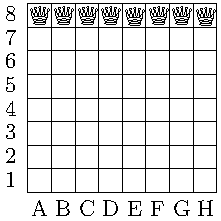
\includegraphics[scale=1]{slides/DomChess8.pdf}}&
      \pause{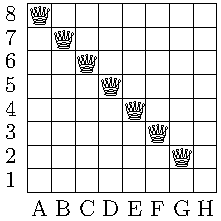
\includegraphics[scale=1]{slides/DomChess7.pdf}}\\
      \pause{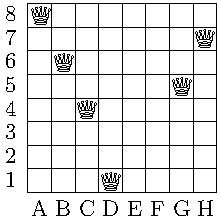
\includegraphics[scale=1]{slides/DomChess6.pdf}}&
      \pause{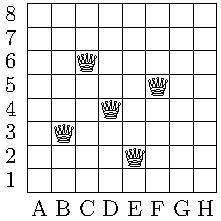
\includegraphics[scale=1]{slides/Chess1.pdf}}
    \end{tabular}
  \end{figure}
\end{frame}

% --------------------------------------------------- Slide --
%\subsection{Figures}
\label{figures2}
\begin{frame}\frametitle{Single figure with caption}
  \begin{figure}[htb]
    \centering
    
\includegraphics[scale=0.25]{slides/figures/400x400.png}
    \caption{This is an caption!}
  \end{figure}
\end{frame}